\chapter{Greifermechanik}
\label{greifer}
\section{Einleitung zur Mechanik}
Ziel der konstruktiven Arbeit am und mit dem Quadrokopter ist ein modular zu montierender Greifarm, welcher mit Kameras und Sensoren sein Ziel selbst finden kann. Dabei ist die Mechanik des Greifarms der Kern der Arbeit und beginnt an der Verbindungsstelle mit dem Motor und endet mit der letztendlichen Kontaktstelle zur Last, welche transportiert werden soll.
\par
Dabei sollte der Fokus der konstruktiven Ausarbeitung eine stabile, funktionssichere, leichte und dauerfeste Konstruktion sein, welche selbst bei nicht idealen Bedingungen ihre Aufgaben erfüllt und dabei insbesondere das Wohlergehen von Passanten nicht gefährdet. Beim Aspekt der Stabilität und Sicherheit ist insbesondere die Greifsicherung im Falle eines Defekts und die Lage des Schwerpunkts zu beachten. Gleichzeitig darf ein maximales Gewicht von 2kg nicht überschritten werden, da sonst ein spezieller Drohnenführerschein als Nachweis zum Bedienen des Quadrokopters nötig ist.
\par 
Für die Konstruktion steht als Grundmaterial für den Rahmen Plexiglas zur Verfügung, welches mit Laserschneidemaschinen in Formen geschnitten werden kann. Weitere benötigte Bauteile wie zum Beispiel ein Motor oder Lagerungen gelten als Zukaufteile.
\par
Die tiefere Forschungsfrage hinter dem Projekt ist die Visualisierung des Greifarms im späteren Verlauf, welche Möglichkeiten einem bei der Konstruktion, beim Leichtbau und der Stabilität mit dem vorausgesetzten Material gegeben sind und wie gut das Konzept umsetzbar ist. Bereits heute gibt es schon erste funktionierende Beispiele, welche durch zum Beispiel große Paketlieferanten und ähnlichen Unternehmen ins Leben gerufen worden sind.
\par
Für die Auswahl eines Konzepts wird zwischen mehreren Prinzipskizzen eine kategorisch ausgewählt und vollständig dimensioniert. Dann wird nochmals die Realisierung geprüft mit einem CAD Modell bzw. Simulation.

\section{Materialien und Vorgaben}
Wie schon in der Einleitung erwähnt, müssen bestimmte Vorgaben eingehalten werden. Die Greifarmmechanik nimmt dabei, wegen ihres großen Bauraumes und im Verhältnis größten Massenanteil, einen sehr großen Teil an Einschränkungen ein.

\subsection{Gesetzeslage}
So liegt die offizielle Gewichtsgrenze für die Nutzung einer Drohne bei 2kg und das Eigengewicht des zur Verfügung gestellten Quadrokopters liegt bei ca. 1,5 kg womit man eine ungefähre Gewichtsgrenze für die Greifarmmechanik plus Last von 500 g hat. So gilt seit dem 07.04.2017 nach Bundesgesetzblatt in Deutschland „...für Besitzer von Drohnen oder Modellflugzeugen mit einem Gewicht von mehr als 2,0 Kilogramm...Darüber hinaus müssen sie besondere Kenntnisse nachweisen. Der Nachweis wird entweder nach Prüfung durch eine vom Luftfahrt-Bundesamt anerkannte Stelle erteilt oder bei Modellflugzeugen durch einen Luftsportverband nach einer Einweisung
ausgestellt.“ \cite{BMVI}. Dabei ist zu beachten das jedes eingesparte Gramm an Gewicht, mehr Laufzeit und demnach mehr Effizienz pro Akkuladung mit sich bringt bzw. umgekehrt eine höhere tragbare Last zur Folge hat.

\subsection{Materialvorgabe}
Um in dieser geringen Gewichtsklasse zu bleiben, wird ein stabiler und gleichzeitig leichter Werkstoff benötigt, welcher zugleich auch keine Unmengen an Kosten mit sich bringt, damit auch der wirtschaftliche Aspekt im Laufe verschiedener Experimente und Testdurchläufe nicht komplett ausgereizt wird. Das Institut bietet dafür Plexiglasplatten an, welche in verschiedenen Wandstärken (3 mm und 6 mm) angeboten werden und zugleich mit einer Laserschneidemaschine in verschiedenste Formen geschnitten werden können. Dabei bietet Plexiglas eine brauchbare Steifigkeit für leichte Anwendungsfälle, sowie mit einer Dichte von 1,18 g/cm³ \cite{Plexiglasdichte} ein geringes Gewicht, wobei es keine enormen Kosten mit sich bringt.

Neben Kunststoffkleber bietet das Institut außerdem, für form- und kraftschlüssige Verbindungen, Schrauben und Muttern in verschiedensten Längen und Durchmessern an. Da es sich hier jedoch um Metall- und keine Kunststoffschrauben handelt, ist während der konstruktiven Auslegung der Greifarmmechanik auf eine geringe Stückzahl zu achten, um ein zu hohes Gewicht zu verhindern.

\section{Aufgabe und Konzeptideen für die Greifarmmechanik}
Die grobe Hauptaufgabe der Greifarmmechanik besteht im Aufnehmen und Ablegen einer Last in Form eines kleinen Paketes, welches mit dem Quadrokopter von einem Ort zum anderen Ort transportiert wird. Dabei sollte eine gewisse Stabilität gegeben sein, sowie eine realistische Sicherheit.

Im Folgenden werden dementsprechend drei Konzeptideen vorgestellt und dessen Vor- und Nachteile gegenübergestellt, wobei dann ein Konzept kategorisch festgelegt wird.

\subsection{1.~Konzept}
Die Funktionsweise des ersten Konzepts aus Abbildung \ref{erste_prinzipskizze} basiert auf einen Motor, der mittels Schnur entgegen einer Feder eine Art Scherensystem öffnet, an denen sich Greifarme befinden, welche die Last halten sollen. Durch die Federkraft soll die benötigte Haftkraft über die Greifarme an die Last geleitet werden, welche ein Abrutschen verhindern soll.
\par
Das Konzept zeichnet sich mit einem relativ simplen Aufbau aus, welcher einen geringen Bauraum einnimmt. Durch die Federkraft wird ein sicherer Halt selbst bei Defekten an der Elektronik gewährt. Die mögliche, aber nicht notwendige, parallele Bauweise kann weitere Stabilität hinzufügen.
Durch die relativ steifen Greifarme, ist eine erhöhte Präzision beim Ansteuern der Last erfordert. Auch die Rutschfestigkeit bei den Greifarmen ist ungewiss und muss experimentell überprüft werden.
Genauso ist die Federdimensionierung und, mit dessen Lebensdauer, die gebotene Haftkraft unsicher.

\begin{figure}[h]
	\begin{center}
	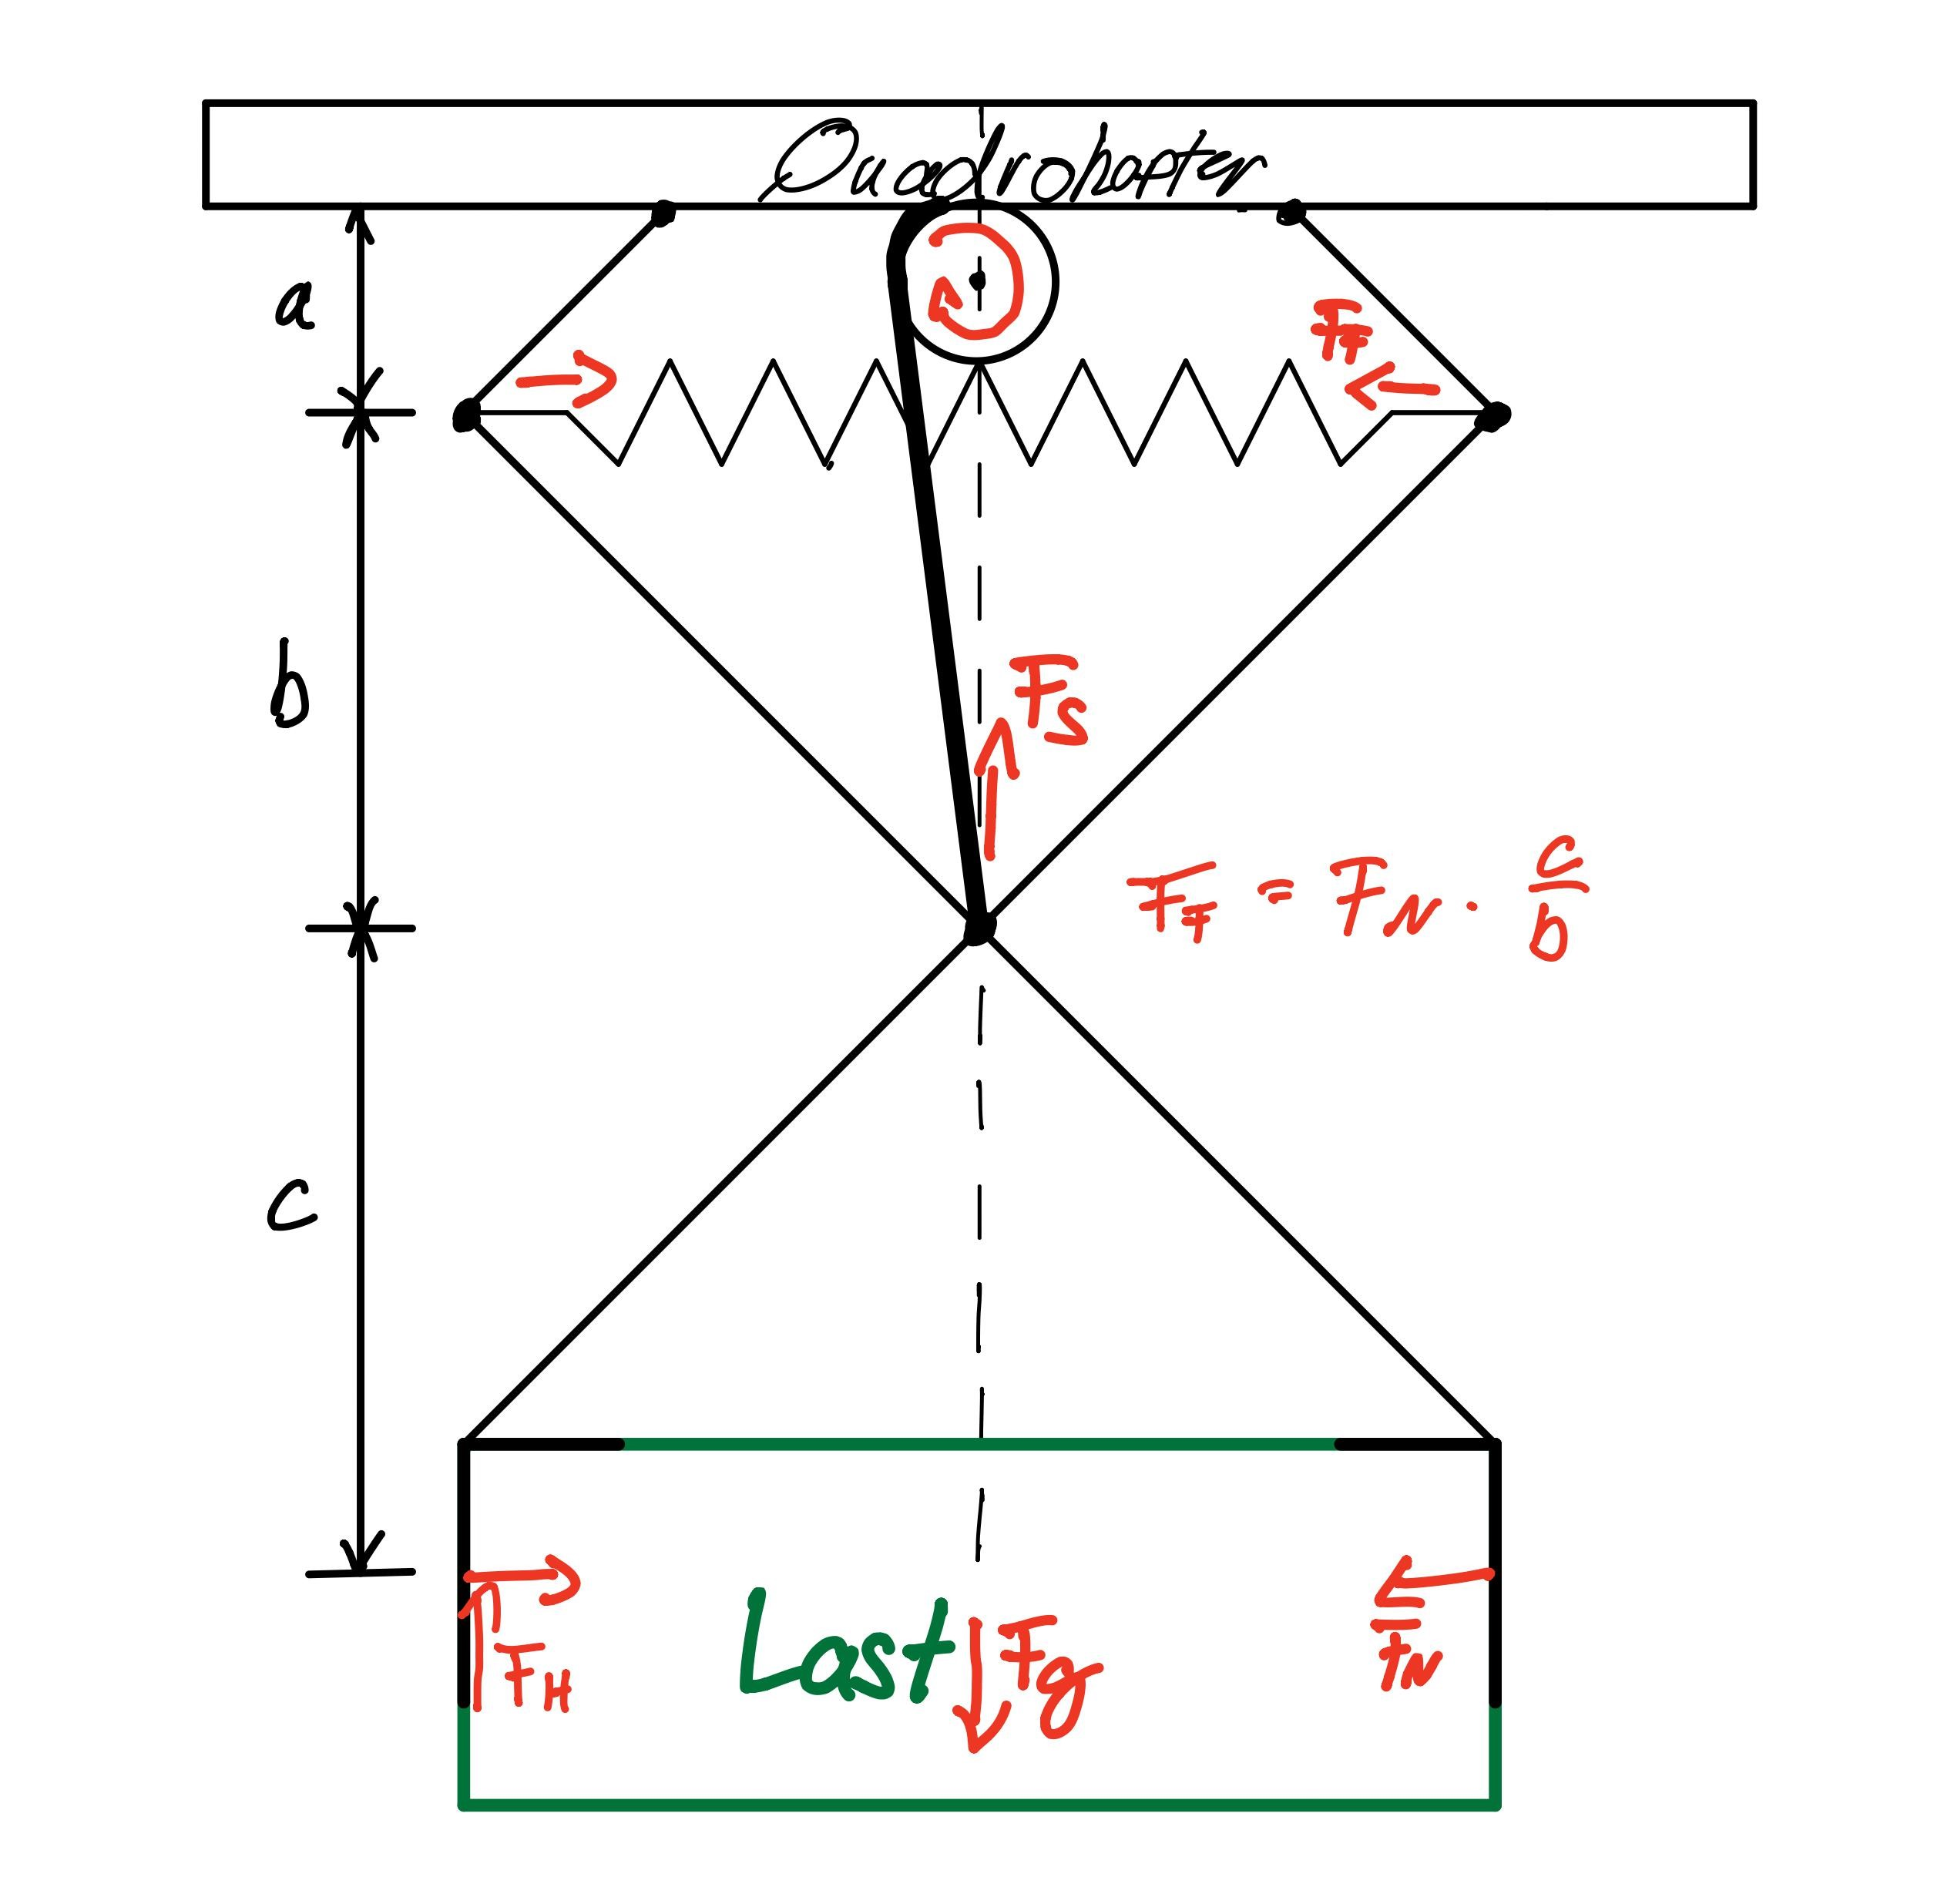
\includegraphics[scale=0.5]{"Grafiken/Skizze1mechanik.png"}
	\caption{Erste Prinzipskizze}
	\label{erste_prinzipskizze}
	\end{center}
\end{figure}

\newpage
\subsection{2.~Konzept}
Bei der Funktionsweise des zweiten Konzepts aus Abbildung \ref{zweite_prinzipskizze} übernimmt ein elektrischer Hubzylinder die Arbeit. Dieser öffnet und schließt Greifarme und hält diese in Position mit seiner eigenen Steifigkeit.
\par
Auch hinter dem zweiten Konzept steckt ein simples Grundprinzip. Vorteil des Hubzylinders wäre die Steifigkeit, die ohne elektrisches Signal nicht schwindet. Auch ist hier eine parallele Bauweise für mehr Stabilität möglich. Durch den einfach geregelten Hubzylinder, lässt sich die Greifarmbreite beliebig einstellen, wodurch verschieden große Pakete aufgenommen werden können.
\par
Jedoch wird trotzdem eine gewisse Präzision beim Ansteuern des Paketes benötigt. Auch ist die Rutschfestigkeit wie beim ersten Konzept nicht gewiss. Zusätzlich wird durch die horizontale Bauweise des Hubzylinders ein großer Bauraum eingenommen.
\begin{figure}[h]
	\begin{center}
	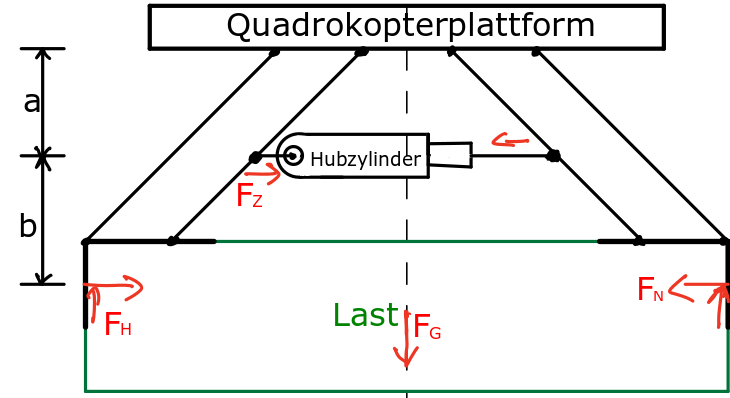
\includegraphics[scale=0.7]{"Grafiken/Skizze2mechanik.png"}
	\caption{Zweite Prinzipskizze}
	\label{zweite_prinzipskizze}
	\end{center}
\end{figure}
\newpage
\subsection{3.~Konzept}
Hinter der Funktionsweise des dritten und letzten Konzepts aus Abbildung \ref{dritte_prinzipskizze} verbirgt sich ein Knickgelenk an dessen Ende ein Magnet ist. Dieses Knickgelenk wird mittels zwei Motoren ausgefahren.
\par
Das letzte Konzept ist zwar, durch den zweiten integrierten Motor, etwas komplexer, jedoch entfällt durch den Magneten die Reibungskomponente, was eine erhöhte Zuverlässigkeit bietet. Auch wird dadurch das Ansteuern des Paketes vereinfacht. Durch das Knickgelenk, kann der Schwerpunkt des gesamten Systems sehr gut mittig gehalten werden.
Jedoch wird die Gesamtmasse durch den zweiten Motor deutlich erhöht, was auch die maximale Paketmasse niedrig hält. Auch ist die letztendliche Kamera- und Sensorpostion nicht wirklich zentrierbar durch die Lage des Knickgelenks

\begin{figure}[h]
	\begin{center}
	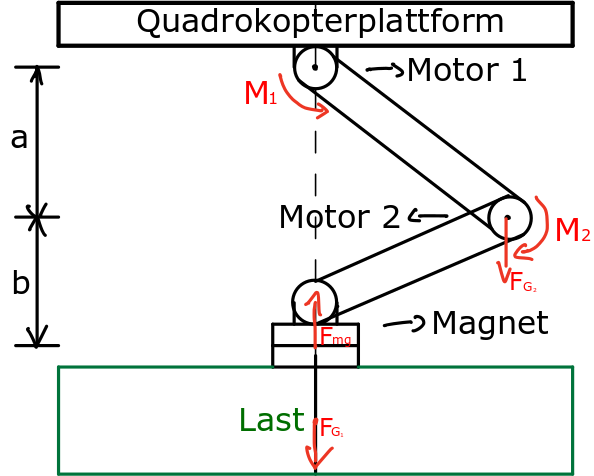
\includegraphics[scale=0.7]{"Grafiken/Skizze3mechanik.png"}
	\caption{Dritte Prinzipskizze}
	\label{dritte_prinzipskizze}
	\end{center}
\end{figure}
\newpage
\subsection{Konzeptauswahl}
Für ein letztendliches Fazit werden Vor- und Nachteile der vorgestellten Konzepte verglichen und abgewogen, um ein finales Konzept auszuwählen.\\
\\
Dabei überzeugt das zweite Konzept aus Abbildung \ref{zweite_prinzipskizze} am meisten, da der Hubzylinder einen stabilisierenden Faktor ins System mit einbringt und sich nur in der Länge verändert, wenn das dafür geeignete Regelgerät das elektrische Signal dafür bekommt. Bei dem ersten Konzept aus Abbildung \ref{erste_prinzipskizze} wäre die konstant benötigte Federkraft zu anfällig auf die anhäufenden Öffnungszyklen. Außerdem sind die simple Bauweise und gleichzeitig stabile Konstruktion des zweiten Konzepts weitere Faktoren, welche für das Konzept sprechen. Gleichzeitig ist ein größerer Spielraum bei der Paketmasse auch ein überzeugender Aspekt, welcher gegen das dritte Konzept aus Abbildung \ref{dritte_prinzipskizze} spricht.\\
\\
Der Hauptfokus liegt demnach im Bauraum und der Länge des elektrischen Hubzylinders, wobei zweiteres als Zukaufteil nicht beliebig variabel ist. Ebenfalls ist die Leistung des Hubzylinders zu beachten, da er bei einem Material wie Plexiglas durchaus in der Lage ist, dieses, bei einem Fehler des Systems, zu zerstören.

\section{Berechnung und Vordimensionierung}
Bei der Berechnung und Vordimensionierung der Greifarmmechanik liegt der Hauptfokus auf dem Bauraum, dem Gewicht des Systems und der letztendlichen benötigten Kraft, welche von dem elektrischen Hubzylinder geleistet werden soll, um das Gewicht fest im Griff zu haben. Ersteres wird durch die Höhe und Lage der Standbeine des Quadrokopters begrenzt. Grobe Messungen ergaben einen Bauraum von  $80\times 80\times130 mm^3$. Dieser lässt sich jedoch durch genaue Formanpassung der Plexiglasteile in die Länge erweitern.

\subsection{Benötigte Normalkraft}
Die letztendlich wichtige Kraft ist die wirkende Hubzylinderkraft, welche in Form der Normalkraft an der Greiffläche wirkt. Letztere lässt sich mittels Reibgesetze berechnen. Da die Greifebene zum tragenden Objekt eben ist, ist die Greifebene zur Horizontalen senkrecht. Die Abbildung \ref{greiferfläche} verdeutlicht die Verteilung der Kräfte.
\begin{figure}[h]
	\begin{center}
	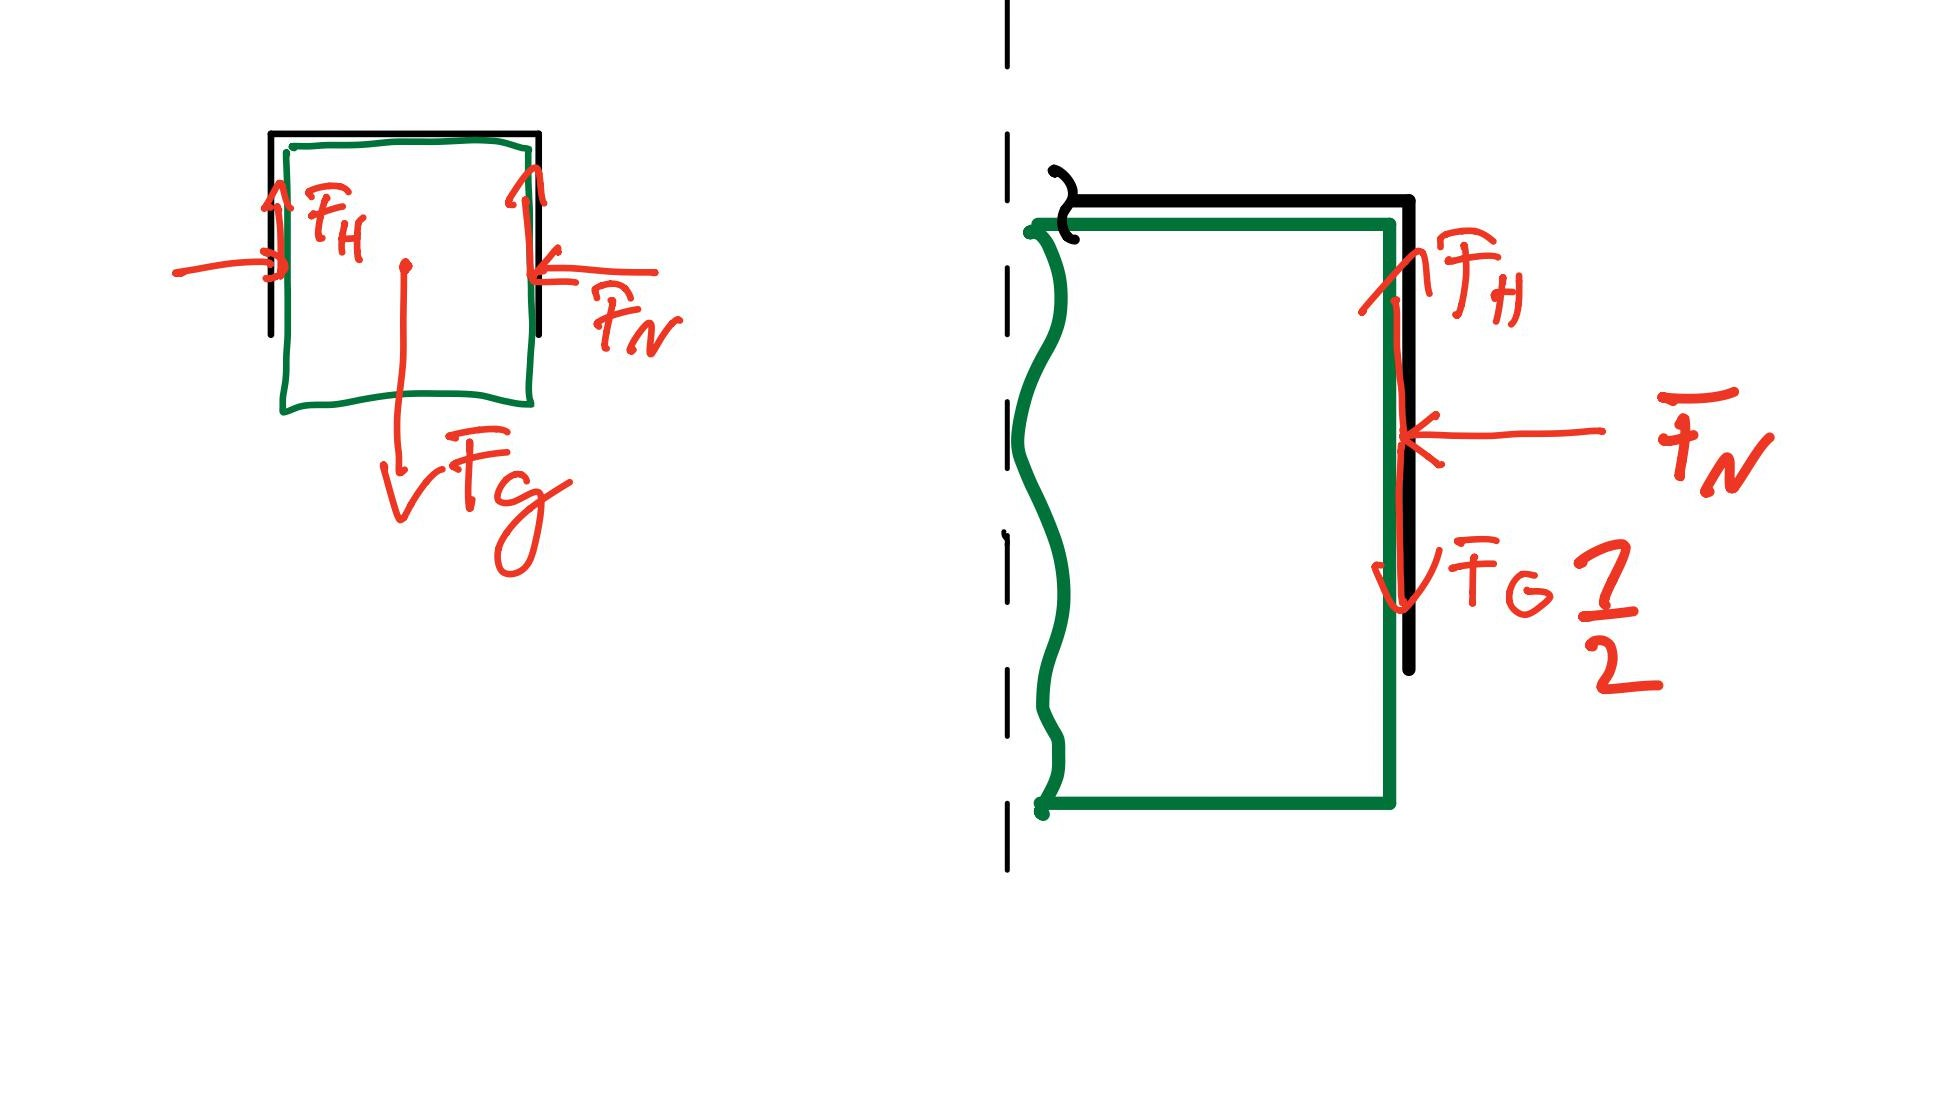
\includegraphics[scale=0.6]{"Grafiken/Greiferflaeche.png"}
	\caption{Kraftverteilung an der Greiferfläche}
	\label{greiferfläche}
	\end{center}
\end{figure}
Aus der Abbildung \ref{greiferfläche} ergibt sich, dass die letztendlich benötigte Normalkraft abhängig von der Gewichtskraft und dem Haftreibwert ist. Da sich die Reibwerte zu jeweiligen Gleitebenen verschiedener Materialien nur experimentell erörtern lassen, muss ein Mittelwert genommen werden, welcher nach den ersten Experimenten eventuell zu korrigieren ist. Als Oberflächen werden Gummi und Plexiglas genommen. Nach längerer Recherche setzt sich ein ungefährer Mittelwert von $\mu_H = 0,3$ durch.\footnote[1]{Quelle für Haftreibungszahlen: https://www.chemie.de/lexikon/Haftreibung.html (23.05.2020)}
\par
\newpage
Für die zu ermittelnde Gewichtskraft ist von einem Gewicht von $m=50g$ bis $m=100 g$ für die Last zu schätzen. Um eine gute Fehlertoleranz und damit Sicherheit zu bieten, wird der errechnete Wert mit dem Faktor $S = 1,8$ angepasst.
Mit dem gegebenen Haftreibwert und der Erdbeschleunigung $g = 9,81 \frac{m}{s^2}$ auf die Last, lässt sich nun die nötige Haftkraft in Form der Normalkraft berechnen:

\begin{eqnarray}
\label{erste_berechnung}
\begin{split}
\frac{1}{2}F_G &= F_H  \\
F_G &= mg \\
F_H &= F_N \times \mu_H \\
mg &= 2 F_N \times \mu_H \\
F_N &= \frac{mg}{2\mu_H} \\
	&= \frac{0,1kg\times9,81\times\frac{m}{s^2}}{2\times 0,3} \\
	&= 1,635N \\
F_{Nmin} &= F_N\times S \\
	&= 1,635N\times 1,8 \\
	&= 2,943N \\
\end{split}
\end{eqnarray}

Aus der Berechnung \eqref{erste_berechnung} ergibt sich also eine ungefähr benötigte Normalkraft von $F_{Nmin} = 3N$.

\subsection{Benötigte Hubzylinderkraft}

Die schlussendlich benötigte Hubzylinderkraft lässt sich über einfache Hebelgesetze mit der Normalkraft schlussfolgern. Anhand der Abbildung \ref{mechanikskizze} und den darauf rotierenden angedeuteten Hebelarmen, erkennt man, dass die maximale Hebellänge in senkrechter Stellung erreicht ist. Die Wahl des Hebelverhältnisses zwischen $a$ und $b$ ist hier entscheidend. Denn Bauraum und Maße der in Frage kommenden Hubzylinder setzen hier starke Grenzen. Für die grobe Vordimensionierung wird das Verhältnis von $a$ zu $b$ auf $1:1$ gesetzt.

\begin{figure}[h]
	\begin{center}
	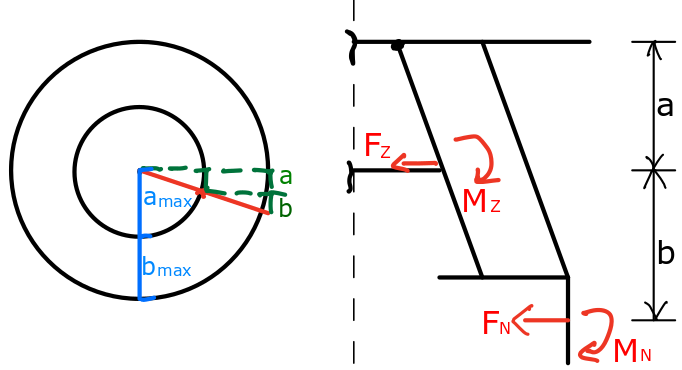
\includegraphics[scale=0.5]{"Grafiken/Mechanikskizze.png"}
	\caption{Kraftverteilung an den Hebelarmen}
	\label{mechanikskizze}
	\end{center}
\end{figure}

\begin{eqnarray}
\label{zweite_berechnung}
\begin{split}
F_N \times(a+b) &= F_Z \times a \\
F_Z &= F_N \times (1 + \frac{b}{a}) \\
 2F_N &= 6N
\end{split}
\end{eqnarray}

\subsection{Auswahl des Hubzylinders}
Mit der in \eqref{zweite_berechnung} berechneten Hubzylinderkraft von $F_Z=6N$ fällt die Wahl des elektrischen Hubzylinders auf den „Titan 30“ von CTI-Modellbau \footnote[1]{Titanzylinder: https://www.cti-modellbau.de/-74-102-110-170-185-328-532.html (23.05.2020)}, welcher mit dem „Thor4HF Titan 1 Regler“, ebenfalls von CTI-Modellbau  \footnote[2]{Titanregler: https://www.cti-modellbau.de/-74-102-110-181-182-191-329-350-543.html (23.05.2020)}, betrieben wird. Durch den begrenzten Bauraum bieten sich nicht viele Alternativen an, da die Firma CTI-Modellbau sich explizit auf den Modellbau konzentriert.
Mit einer erwünschten Öffnungsbreite von jeweils 30 mm pro Seite und einem Faktor von 2, durch die mittige Position des Hubzylinders, lässt sich eine erwünschte Hublänge von 30 mm errechnen.

\section{Vom Modell zu den ersten Bauteilen}
\subsection{Creo Modell}
Mit den ersten vordimensionierten Bauteilen und den ersten festen Maßen von den Zukaufteilen, lässt sich nun ein erstes 3D CAD-Modell bauen. Dabei werden je nach Absprache und Änderungen von Eigenschaften Anpassungen unternommen, um dem finalen Produkt so nah wie möglich zu ähneln. Aus dem CAD Modell aus Abbildung \ref{creo1}, modelliert mit "Creo Parametrics5", lässt sich schon die grobe Gestalt der Greifarmmechanik erkennen.
\newpage
Ausgehend von der Nummerierung in Abbildung \ref{creo1} erkennt man die Bauteile Bodenplatte(1), Hebelarm(2), Führungsschiene(3) und Greifplatte (4). Sie bilden die Grundbausteine des Endprodukts der Greifarmmechanik. Im Zwischenraum von Bodenplatte und Hebelarmen soll später der Hubzylinder(5) Platz finden. Bauteile wie zum Beispiel Verbindungsschrauben oder Abstandshülsen sind außen vor und werden erstmal nicht in der Auflistung berücksichtigt, da diese sich in der Anzahl und der Position noch stark ändern können.
\begin{figure}[h]
	\begin{center}
	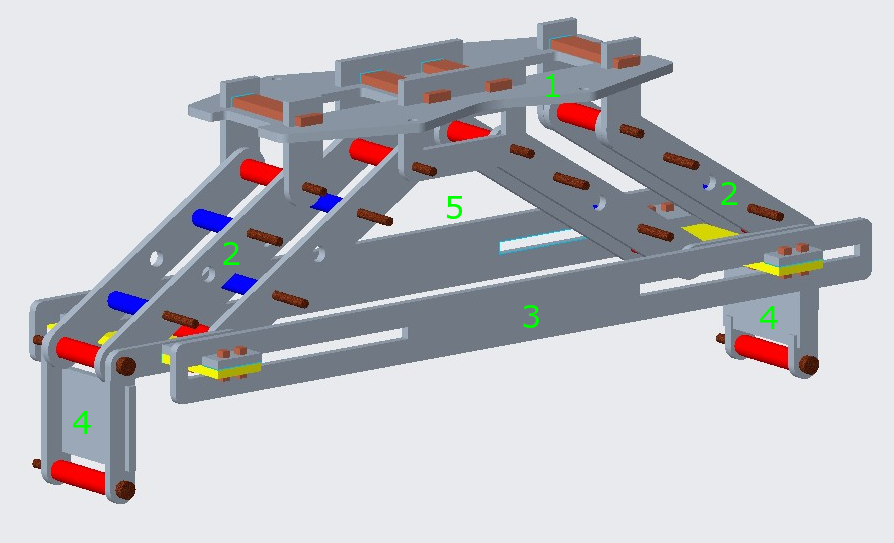
\includegraphics[scale=0.6]{Grafiken/Creo1bearbeitet.png}
	\caption{Erstes CAD-Modelle}
	\label{creo1}
	\end{center}
\end{figure}
\subsection{Inkscape}
Die letztendlich fertigen dreidimensionalen CAD-Bauteile können nun mit „Inkscape“, eine Software zur Bearbeitung und Erstellung zweidimensionaler Vektorgrafiken, zu Schnittmustern erzeugt werden. Mithilfe dieser Schnittmuster werden die fertigen Bauteile zweidimensional aus den Plexiglasplatten mit konstanter Wandstärke von der Laserschneidemaschine ausgeschnitten. Dementsprechend ist bei der Konstruktion der Bauteile zu beachten, dass diese zweidimensional als Schnittmuster abgebildet werden können.

\begin{figure}[h]
\begin{center}
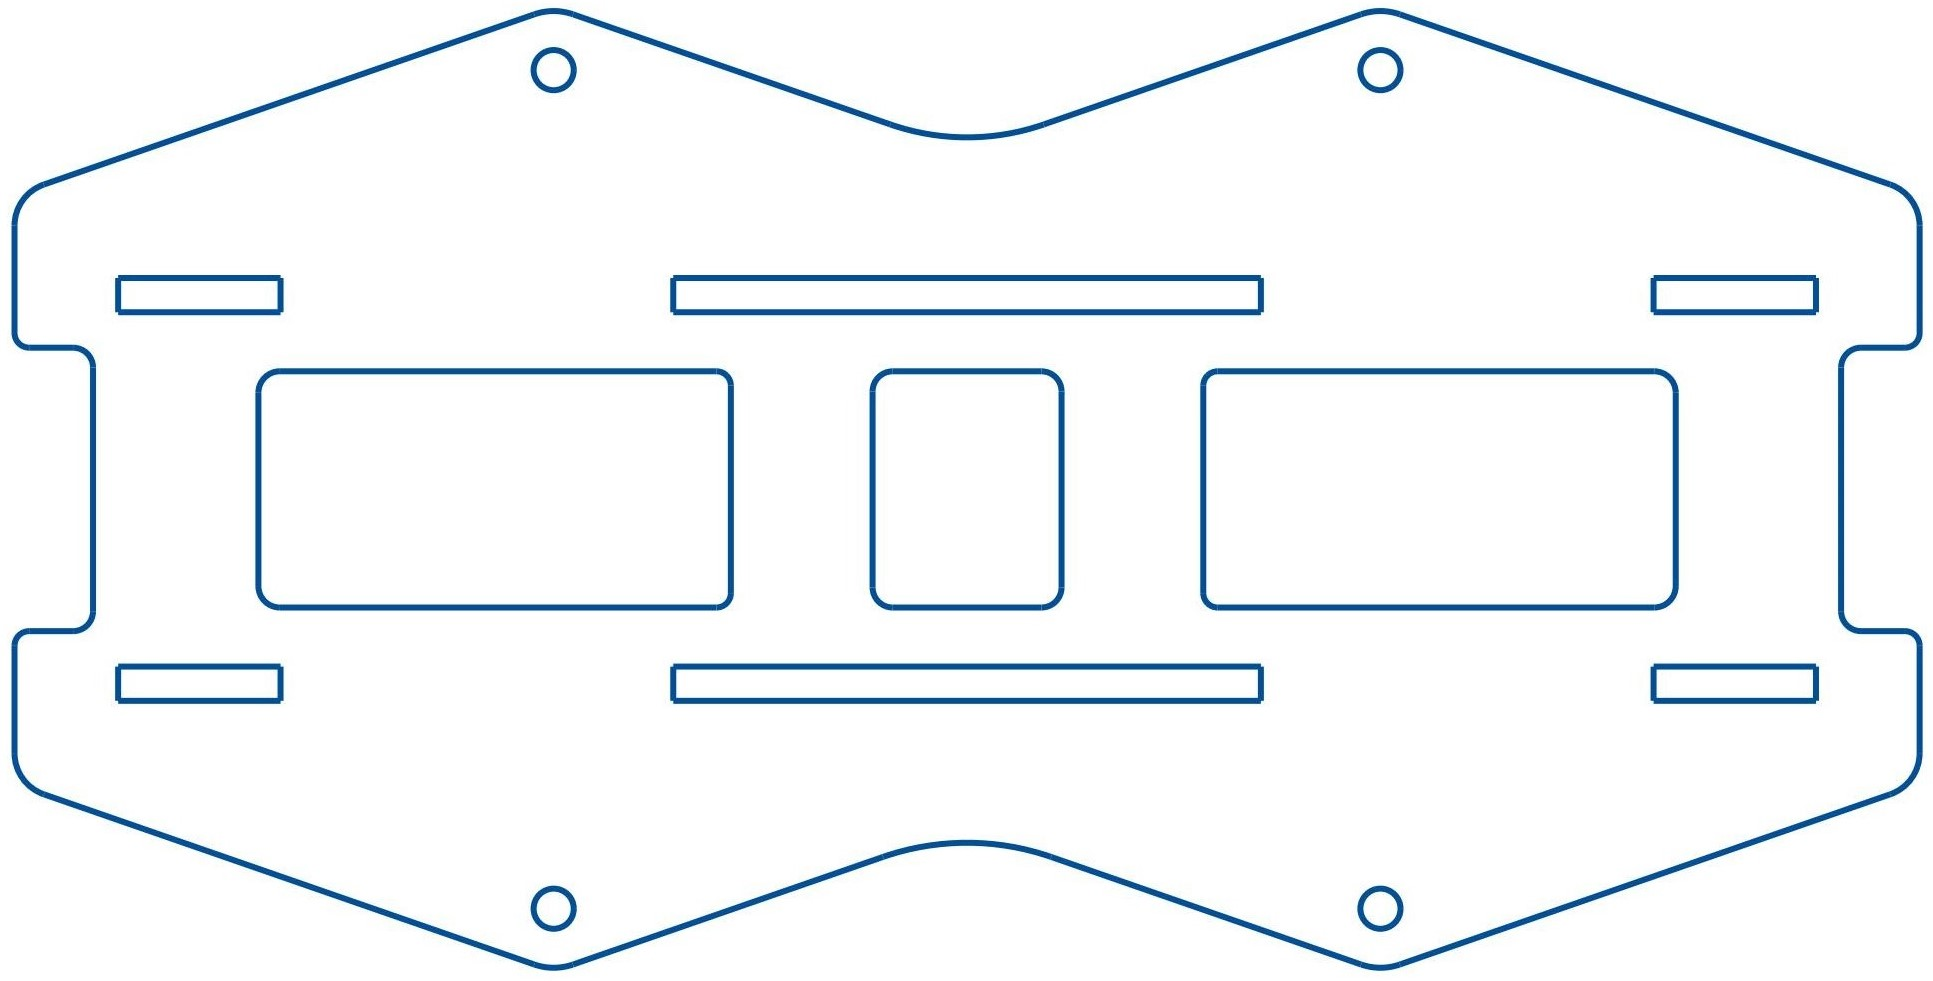
\includegraphics[scale=0.5]{Grafiken/Inkscapebodenplatte.jpg}
\caption{Inkscapeschnittmuster der neuen Bodenplatte}
\label{inkscape1}
\end{center}
\end{figure}

\subsection{Erste Ergebnisse}
Die ausgeschnittenen Bauteile werden zur Probe vormontiert, um mögliche Problemstellen ausfindig zu machen. Die Abbildungen \ref{hebelarme} und \ref{vormontage} zeigen erste Montageversuche.

\begin{figure}[h]
\begin{center}
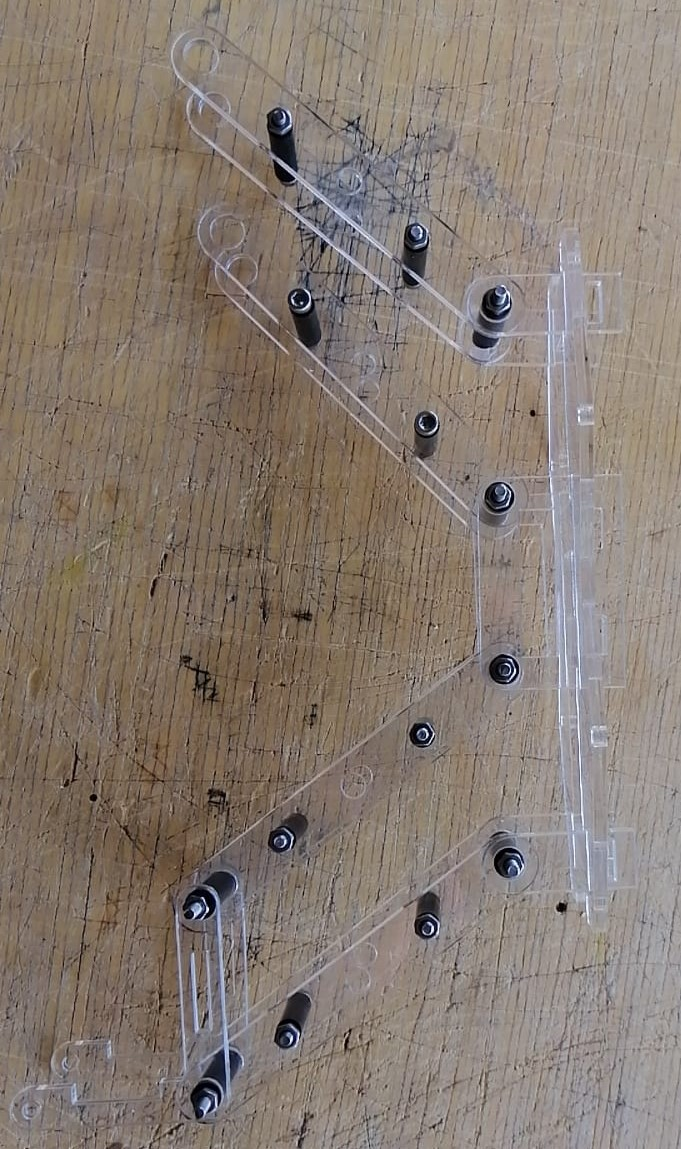
\includegraphics[angle=90,scale=0.3]{Grafiken/Fotohebelarme.jpg}
\caption{Zusammengebaute Hebelarme}
\label{hebelarme}
\end{center}
\end{figure}

\begin{figure}[h]
\begin{center}
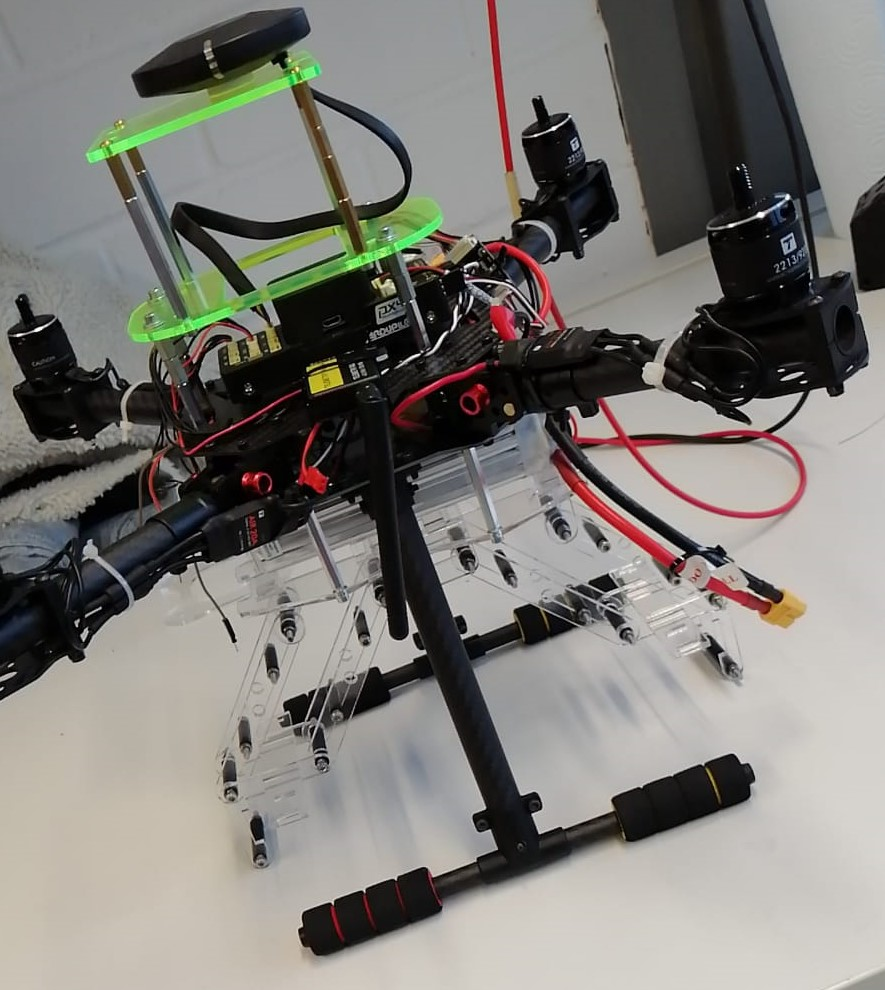
\includegraphics[scale=0.4]{Grafiken/Fotoquadrokopter.jpg}
\caption{Vormontage der Greifarmmechanik am Quadrokopter}
\label{vormontage}
\end{center}
\end{figure}
Um die aus den Berechnungen gewünschte Reibung zu erlangen wird auf den Flächen der Greiferplatten (Nummer 4 in Abbildung \ref{creo1}) noch eine Gummischicht draufgeklebt.
Nach der letztendlich fertigen Konstruktion muss für die Sensoren noch eine Befestigung hinzugefügt werden. Diese ist aber letztendlich stark vom eingenommenen Volumen des Greifsystems im Bauraum abhängig, da sie bestenfalls zentriert liegt und wird erst nach den ersten Testläufen beigefügt

\section{Problematiken und Lösungen}
Bei den ersten Testläufen ist vermehrt aufgefallen, dass die Wandstärken mit dem CAD Modell schlecht einschätzbar sind und demnach lange und dünne Bauteile wie zum Beispiel die Führungsschienen (Nummer 3 in Abbildung \ref{creo1}) so umkonstruiert werden müssen, damit die gewollte Steifigkeit von dem benutzten Plexiglas trotzdem noch erhalten bleibt.\\
\\
Gleichzeitig muss auf die Anziehkraft der Schrauben geachtet werden, da bei zu hohen Kräften das Plexiglas durchbrechen könnte oder auch zu hohen Reibungskräften unterliegen würde, welche das System zu sehr unkontrolliert beeinflussen würde. Demnach sind alle Schrauben nicht komplett versteift eingeschraubt, was gleichzeitig zur Folge hat, dass Steifigkeit und Stabilität des Systems in gewissen Maßen drunter leiden. \\
\\
Auch funktioniert die Führungsschiene nicht so wie angedacht, da zu hohe Reibungskräfte zwischen den einzelnen Plexiglasflächen entstehen. Ein kurzer Umbau lässt nun die Führungsschiene das System, über die schon angebrachten Bolzen, an den Greifern führen. Auch diese Lösung ist nicht perfekt, denn wenn die Querkräfte zu hoch werden, verbiegt sich das Plexiglas und erfüllt demnach nicht mehr seine Funktion einwandfrei. Auch das ist mit einer erhöhten Wandstärke auf Kosten höheren Gewichts teilweise besser geworden. Da aber auch hier die Reibung zwischen Führungsbolzen und Plexiglas nicht komplett zu verhindern ist, lässt sich das Problem nicht ganz lösen.\\
\\
Ein weiteres Problem ist der Öffnungswinkel des Systems. Denn um 60 mm gewollten Öffnungsspalt zu erreichen, müssten die Hebel weiter voneinander entfernt liegen, was das Volumen des Greifarms noch größer machen würde. Denn die Länge des Hubzylinders ist nicht stark variabel, weshalb der Bauraum zur Mitte hin begrenzt ist. Der momentane Öffnungsspalt von 45 mm sollte demnach erstmal beibehalten werden, da Verbesserungen größere Maßnahmen erfordern würden.
\section{Fazit zur Mechanik}

Bei der letztendlichen Fertigstellung der Mechanik zeigt sich die Komplexität darin die Balance zwischen Leichtbau, Stabilität und Steifigkeit beizubehalten, ohne dabei die Funktion des Greifarms einzuschränken und das mit einfachsten Mitteln. Der Verzicht auf einen Elektromagneten für die Greiffunktion führt zu einem großen eingenommenen Bauraum und viel Zusatzgewicht, da die Konstruktion der Greifarme für die anliegenden Kräfte eine gewisse Stabilität brauchen. In realitätsnahen Szenarien werden Faktoren wie zuverlässige Stabilität und möglichst lange Akkulaufzeiten jedoch benötigt. Dies stellt sich als eine zukünftige Hürde für andere Projekte dieser Art heraus. Die Grundfunktion an sich wird jedoch erfüllt.\\
\\
Das Bauen ohne zuverlässige Lagerung erwies sich auch nicht als einfach und kostete dem System weitere Stabilität. Auch der enorme Bauraum, generiert durch den Hubzylinder, setzt dem System starke Grenzen und führt zu einem erhöhten Gewicht.
